% $Id: $
\documentclass[a4paper,12pt]{article}
\usepackage{a4wide}
\usepackage{enumerate}
\usepackage{amsmath,amsthm,amssymb}
\usepackage{amsfonts}
% The following makes latex use nicer postscript fonts.
\usepackage{times}
\usepackage{subcaption}
\usepackage[english]{babel}
\usepackage{tikz}
%\usepackage[colorlinks,urlcolor=blue,linkcolor=blue]{hyperref}
\pagestyle{headings}
\newcommand{\upuparrow}{\mathrel{\reflectbox{\rotatebox[origin=c]{90}{$\twoheadrightarrow$}}}}
\newcommand{\downdownarrow}{\mathrel{\reflectbox{\rotatebox[origin=c]{90}{$\twoheadleftarrow$}}}}
\usepackage{vubtitlepage}
\usepackage{lmodern}
\usepackage{graphicx}

\usepackage[geometry]{ifsym}
%\usepackage[font=small,format=plain,labelfont=bf,up,textfont=it,up]{caption}
\renewcommand{\thefigure}{\thesection.\arabic{figure}}
\author{Filip Moons}
\title{Tiny Compiler}
%\theoremstyle{definition}
\newtheorem{theorem}{Theorem}[section]
\newtheorem{lemma}[theorem]{Lemma}
\newtheorem{proposition}[theorem]{Proposition}
\newtheorem{conjecture}{Conjecture}
\newtheorem{example}[theorem]{Example}
\newtheorem{property}[theorem]{Property}
\newtheorem{definition}[theorem]{Definition}
\newtheorem{corollary}[theorem]{Corollary}
\newtheorem{remark}[theorem]{Remark}
\newtheorem{examples}[theorem]{Examples}
\newtheorem{remarks}[theorem]{Remarks}
\newtheorem{notation}[theorem]{Notation}
\setcounter{tocdepth}{5}
\newcommand{\N}{{\mathbb N}}
\newcommand{\Z}{{\mathbb Z}}
\newcommand{\Q}{{\mathbb Q}}
\newcommand{\R}{{\mathbb R}}
\newcommand{\C}{{\mathbb C}}
\newcommand{\HQ}{{\mathbb H}}
\renewcommand{\P}{{\mathbb P}}
\newcommand{\E}{{\mathbb E}}
\newcommand{\cost}{\text{cost}}
\newcommand{\Nash}{\text{Nash}}
\newcommand{\nash}{\text{nash}}
\newcommand{\opt}{\text{opt}}
\newcommand{\LFP}{\text{LFP}}
\renewcommand{\int}{\text{int}}

%\newenvironment{proof}{\noindent{\bf Bewijs.}}{{\hfill $ \ Box $}\vskip 4mm}

\promotortitle{Professor:}
\promotor{Prof. Dr. D. Vermeir}
\advisors{}
\advisortitle{}
\addto\captionsenglish{\renewcommand*\abstractname{Abstract for non-mathematicians}}
\date{MEI 2006}
\faculty{Faculty of Science}
\advisortitle{}
\department{Master in Applied Computer Science}
\reason{Project of the course `Compilers'}

\date{September 2014}


\begin{document}
% Then english TitlePage
\maketitlepage


\tableofcontents
\newpage
% \pagenumbering{arabic}
\section{Introduction}
This paper gives the complete construction of the Scott topology. The Scott topology was first defined by Dana Scott for complete lattices, but later a toned construction of the Scott topology is defined on a posets with some necessary properties.

An introduction to order theory is given in the second section. In this section, the most  important definitions and properties on posets needed for the rest of this paper, are stated. The concept of the ``Way Below''-relation, a much stronger relation than the ordinary `less than or equal to', is also introduced here. 

The next section is about Scott convergence. We introduce lower limits on posets and with this concept, we can give meaning to a certain convergence of nets, the Scott convergence. Using the general relation between convergence and topology, the notion of Scott convergence will lead to the construction of the Scott topology. Some nice properties of the Scott open sets are also shown here.

The second last section is about Scott continuous functions. A function between posets is Scott-continuous if and only if it is continuous with respect to the Scott topology. It will become clear that such functions are always monotone and preserve the directness-property of directed sets. This means that the Scott continuity can also be express in lattice theoretical terms. A nice fixed-point theorem for Scott-Continuous functions is also included here.

The concluding section discusses some categorical theory to search for topological spaces that we can become by considering the Scott topology on a continuous lattice. This gives rise to a beautiful conclusion: the Scott-topology on a continuous lattice is always an injective $T_O$-space and, conversely, if we consider an injective $T_0$-space, we can construct a continuous lattice if we use a certain order (the specialization order). More mathematically, we show that $INJ$, the full subcategory of $TOP$ consisting of injective spaces and all continuous maps, is essentially the same category as $CONT$, the category of all continuous lattices.

One may wonder whether there are applications of the Scott topology. There a lot of applications in theoretical computer science. In the study of models for lambda calculi and the denotational semantics of computer programs, the Scott topology appears very often.

\newpage
\section{Order theory}
\subsection{Ordered sets}
\subsubsection{Preordered sets}
\begin{definition} Consider a set $L$ equipped with a reflexive and transitive relation $\leq$. Such a relation will be called a \emph{preorder} and $L$ a \emph{preordered set}. A subset $D$ of $L$ is \emph{directed} provided it is nonempty and every finite subset of $D$ has an upper bound in $D$. (Aside from non-emptiness, it is sufficient to assume that every pair of elements in $D$ has an upper bound in $D$.) Dually, we call a nonempty subset $F$ of $L$ filtered if every finite subset of $F$ has a lower bound in $F$.
\end{definition}

The notation $x = \bigvee^{\uparrow} X$ is convenient to express that, firstly, the set $X$ is directed and, secondly, $x$ is its least upper bound. \\

Let $L$ be a set with a preorder $\leq$, for $X \subseteq L$, and $x \in L$ we write:
\begin{enumerate}
  \item $\downarrow X = \{y \in L: y \leq x$ for some $x \in X\}$,
  \item $\uparrow X = \{y \in L: x \leq y$ for some $x \in X\}$,
  \item $\downarrow x = \downarrow\{x\}$,
  \item $\uparrow x = \uparrow\{x\}$,
  \item X is a \emph{lower set} iff $X = \downarrow X$,
  \item X is an \emph{upper set} iff $X = \uparrow X$,
  \item X is an \emph{ideal} iff it is a directed lower set,
  \item X is an \emph{filter} iff it is a filtered upper set,
\end{enumerate}

\subsubsection{Partially ordered sets}
\begin{definition}
A \emph{partial order} is a transitive, reflexive and antisymmetric relation $\leq$, which means that $x \leq y$ and $y \leq x$ always imply $x = y$. A \emph{partially ordered set} or a \emph{poset} for short, is a nonempty set $L$ equipped with a partial order $\leq$.
\end{definition}

\subsubsection{Chains}
\begin{definition}
A \emph{total order} is a transitive, antisymmetric and total relation $\leq$, which means that for each two elements $a,b$ always holds that $a \leq b$ or $b \leq a$. A totally ordered set $L$ is also called a \emph{chain}.
\end{definition}


\subsection{Nets}
\begin{definition}
A \emph{net} in a set $X$ is a function
$$N: J \rightarrow X : j \mapsto x_j$$
whose domain $J$ is a directed set. (Nets will also be denoted by $(x_j)_{j\in J}$ or just by $(x_j)$) If the set $X$ also carries a preorder, then the net $x_j$ is called \emph{monotone} if $i \leq j$ always implies $x_i \leq x_j$.
\end{definition}

\subsubsection{Link with filters}
Given a filter $\mathcal{F}$ on $J$, then we determine a net as follows:\\
Consider the following set:
$$L_\mathcal{F} := \{(x,F)|x\in F, F\in\mathcal{F}\}$$
with the order
$$(x,F) \leq (y, G) \Leftrightarrow G \subset F,$$
then
$$N_\mathcal{F}: L_\mathcal{F} \rightarrow X: (x, F) \mapsto x$$
is a net in X.\\

Conversely, given a net $N: J \rightarrow L: l \mapsto x_l$, then we get a filter
$$\mathcal{F}_N := \{F \subset X | \exists l \in L: \{x_n | n \geq l\} \subset F\} $$

Note that $\mathcal{F}_{N_\mathcal{F}} = \mathcal{F}.$

\subsection{Lattices \& dcpo's}
\begin{definition}
An \emph{inf semilattice} is a poset $S$ in which any two elements $a$, $b$ have an inf, denoted by $a \wedge b$. Equivalently, an \emph{inf semilattice} is a poset in which every nonempty finite subset has an inf. A \emph{sup semilattice} is a poset $S$ in which any two elements $a, b$ have a sup $a \vee b$ or, equivalently, in which every nonempty finite subset has a sup. A poset which is both an \emph{inf semilattice} and a \emph{sup semilattice} is called a \emph{lattice}.
\end{definition}

As we will deal with \emph{inf semilattices} very frequently, we adopt the shorter expression `\emph{semilattice}' instead.

If a poset $L$ has a greatest element, it is called the \emph{unit} or \emph{top} element of \emph{L} and is written as $1$. The top element is the inf of the empty set. If $L$ has a smallest element, it is called the \emph{zero} or \emph{bottom} element of \emph{L} and is written 0.

\begin{example}
For any set $X$, the collection of all subsets of A (the power set $2^X$) can be ordered via subset inclusion. This forms a lattice with $\emptyset$ as zero element and with unit $X$.
\end{example}
\begin{example}
Let $X$ be a topological space, then the collection $\mathcal{O}(X)$ of open sets is a partial ordered set for the inclusion relation ($\subseteq$). $\mathcal{O}(X)$ is closed for finite intersections and for all unions. This results in a lattice with unit $X$ and zero element $\emptyset$.
\end{example}

\begin{definition}
\begin{enumerate}
  \item A poset is said to be \emph{complete with respect to directed sets} (shorter: directed complete) if every directed subset has a supremum. A \textbf{d}irected \textbf{c}omplete \textbf{po}set is called a \textbf{dcpo}. A \textbf{dcpo} with a least element is called a \emph{pointed} \textbf{dcpo} or a \textbf{dcpo} with a \emph{zero} element.
  \item A poset which is a semilattice and directed complete will be called a \textbf{directed complete semilattice}.
  \item A \textbf{complete lattice} is a poset in which \emph{every} subset has a sup and an inf. A \emph{totally ordered complete lattice} is called a \textbf{complete chain}.
  \item A poset is called a \textbf{complete semilattice}  iff every nonempty subset has an inf and every directed subset has a sup.
  \item A poset is called \textbf{bounded complete}, if every subset that is bounded above has a least upper bound. In particular, a bounded complete poset has a smallest element, the least upper bound of the empty set.
\end{enumerate}
\end{definition}

\begin{example}
Let $\mathfrak{T}$ be the set of all topologies on a set X, the inclusion relation ($\subseteq$) is a partial order on the set $\mathfrak{T}$ (Remember that for two topologies $\mathcal{T}_1, \mathcal{T}_2$, when $\mathcal{T}_1 \subset \mathcal{T}_2$ then $\mathcal{T}_1$ is said to be coarser and $\mathcal{T}_2$ is said to be finer than $\mathcal{T}_1$). The couple $(\mathfrak{T}, \subseteq)$ defines a lattice. More specific:
\begin{enumerate}
  \item The discrete topology is the unit in $(\mathfrak{T}, \subseteq)$,
  \item The trivial topology is the zero element in $(\mathfrak{T}, \subseteq)$,
  \item If $\mathfrak{G} \subseteq \mathfrak{T}, \mathfrak{G} \neq \emptyset$, then $\bigcap \mathfrak{G}$ is the infimum of $\mathfrak{G}$.

  \item If $\mathfrak{G} \subseteq \mathfrak{T}, \mathfrak{G} \neq \emptyset$, then the topology generated by $\bigcup \mathfrak{G}$ is the supremum of $\mathfrak{G}$.
\end{enumerate}
\end{example}

\begin{example}
$\N$, ordered by divisibility ($a \leq b$ if $a$ divides $b$) forms a complete lattice. The zero element of this lattice is $1$, since it divides any other number. The unit is 0, because it can be divided by any other number. The supremum of finite sets is given by the least common multiple and the infimum by the greatest common divisor. For infinite sets, the supremum will always be 0 while the infimum can indeed be greater than 1. For example, the set of all even numbers has 2 as the greatest common divisor. If 0 is removed from this structure it remains a lattice but ceases to be complete.
\end{example}

\begin{example}
For any poset, the set of all non-empty filters, ordered by subset inclusion, is a \textbf{dcpo}. Together with the empty filter it is also pointed. If the order has binary meets, then this construction (including the empty filter) actually yields a complete lattice.
\end{example}

\begin{property}\label{directeproducten}
The direct product $\prod_{j\in J}L_j$ of a family dcpo's $L_j, j \in J$ is itself a \textbf{dcpo} for the pointwise ordering ($a, b \in \prod_{j\in J}L_j: a \leq b \Leftrightarrow a_j \leq_j b_j \forall j \in J$).
\end{property}

\begin{proof}
The direct product  $\prod_{j\in J}L_j$  with the pointwise ordering is a poset, because the pointwise order relation $\leq$ is a partial order: take $a \in \prod_{j\in J}L_j$, than $a_j \leq_j a_j \forall j \in J \Rightarrow a \leq a$, which shows reflexivity. The transitivity and antisymmetry are shown in the same way.

Now we have to proof that this poset is directed complete. Take a directed subset $D$ of $\prod_{j\in J}L_j$, we have to show that this $D$ has a supremum. If we can prove that for every $j \in J$, the projected subset $D_j = \{d_j | d \in D\}$ of $L_j$ is also directed, then this result follows trivially by definition of the pointwise ordering: because of the fact that $D_j$ has a supremum $y_j$ ($L_j$ is a dcpo), it's clear that $(y_j)_{j \in J}$ is then the supremum of $D$. $D_j$ is nonempty because otherwise $D$ would be empty, which is impossible because $D$ is directed. Take a finite subset $E_j$ of $D_j$, for every $e_j \in E_j$, take an element $(x_i)_{i \in J} \in D$ such that $x_i = e_j$ if $i = j$ and let $E$ be the set of all these elements. Note that this $E$ is a subset of $D$ and that $|E| = |E_j|$, so $E$ is finite. Because $D$ is directed, $E$ has an upper bound $(z_i)_{i \in J}$ in $D$. By the definition of the pointwise ordering, this means that $z_j$ is a valid upper bound for $E_j$. So $D_j$ is directed.
\end{proof}


\subsection{The ``Way Below''-relation}\label{waybelow}
The relations between elements of a given poset are often much stronger than the simple less-than-or-equal-to relation of the partial ordening. For example, consider the lattice $\mathcal{O}(X)$ of open sets of a topological space $X$. To say $U \subseteq V$, but $U \neq V$ does not say very much, since the sets could differ at only one single point! To say that $U$ really is \emph{inside} $V$ it's clear that we need a much stronger relation. 

\begin{definition}
Let $L$ be a poset. We say that $x$ \emph{is way below} $y$, in symbols $x \ll  y$, iff for all directed subsets $D \subseteq L$ for which sup $D$ exists, the relation $y \leq \sup D$ always implies the existence of a $d \in D$ with $x \leq d$. An element satisfying $x \ll x$  is said to be \emph{compact}. The \emph{subset of all compact elements} is denoted by $K(L)$
\end{definition}

In analogy to Definition 1.1, we write
$$\downdownarrow x =  \{u \in L: u \ll x \}$$
$$\upuparrow x =  \{v \in L: x \ll v \}$$


\begin{property}\label{wayprop}
In a poset $L$ the follwing statements hold for all $u, x, y, z \in L$:
\begin{enumerate}[(i)]
    \item $x \ll y \Rightarrow x \leq y$,
    \item $u \leq x \ll y \leq z \Rightarrow u \ll z$,
    \item $x \ll z$ and $y \ll z$ imply $x \vee y \ll z$ whenever the least upper bound $x \vee y$ exists in L,
    \item $0 \ll x$ whenever $L$ has a smallest element $0$.
\end{enumerate}
\end{property}
\begin{proof}
For (i) take the directed family $\{y\}$. The statements in (ii) and (iv) are trivial. For (iii), let $z \leq \sup D$ for a directed set $D$. Then $x \leq d_x$ and $y \leq d_y$ for some $d_x, d_y \in D$, and then $x \vee y \leq d$ for some $d \in D$ larger than $d_x$ and $d_y$.
\end{proof}

\begin{property}\label{opmerkingway}
In a complete semilattice $L$, the way-below relation can be defined equivalently: \\

\noindent $x\ll y$ iff for every subset $X \subseteq L$, the relation $y \leq \sup X$ always implies the existence of a finite subset $A \subseteq X$ such that $x \leq \sup A.$
\end{property}
\begin{proof}
If $y \leq \sup X$, consider the directed set $X^{+} = \{\sup A | \text{A is a finite subset of X} \}$ for which $\sup X^{+} = \sup X$. Thus, if $x \ll y$ in the sense of the definition of the way-below relation, then there is a finite subset $A \subseteq X$ such that $x \leq \sup A$. The converse is immediate.
\end{proof}


\begin{example}
Let $X$ be a topological space and $\mathcal{O}(X)$ be the complete lattice of open sets in $X$.  Suppose $U,V \in \mathcal{O}(X)$ and define the order $\leq$ as the inclusion relation $\subseteq$, then
\begin{align*}
 U \ll V \Leftrightarrow &\forall \mathcal{G} \text{ open cover of } V,\\
 &\exists \mathcal{G}' \subseteq \mathcal{G} \text{ finite cover of } U.
\end{align*}
Indeed, let  $U \ll V$ and take an open cover $\mathcal{G}$ of $V$, $\mathcal{G}$ is a subset of $\mathcal{O}(X)$ with supremum $\cup \mathcal{G}$, the definition of a cover implies $V \subseteq  \cup \mathcal{G}$, and by the way-below relation defined in property\ref{opmerkingway} this always implies the existence of a finite subset $\mathcal{G}' \subseteq \mathcal{G}$ such that $U \subseteq \cup\mathcal{G}'$. Thus $\mathcal{G}'$ is a finite subcover of $U$.

Conversely, if for all open covers $\mathcal{G}$ of $V$ it holds that there exists a finite  subcover $\mathcal{G}'$ of $U$, the characterization follows quite trivially by property \ref{opmerkingway}: consider a subset $\mathcal{D}$ of $\mathcal{O}(X)$ with the relation $V \subseteq \sup \mathcal{D}$, then $\mathcal{D}$ is an open cover of V. Indeed, $\mathcal{D}$ is open because it is a subset of $\mathcal{O}(X)$, so the elements of $\mathcal{D}$ are open sets. It's a cover because $V \subseteq \sup \mathcal{D}$ means $V \subseteq \cup D$. Now it's given that there exists a finite subset $\mathcal{G}'$ of $G$ with $U \subseteq \sup \mathcal{G}'$, so $U \ll V$.

There is also another nice property following from this characterization of the way-below relation: if there is a compact subset $C$ such that $U\subseteq C \subseteq V$, then $U\ll V$. Indeed, every open cover of $V$ is an open cover of $C$, and  since $C$ is compact, finitely many of the covering sets already cover $C$, hence $U$. Thus $U \ll V$.

This example was also to motivation to introduce the ``Way Below''-relation (see introduction of \ref{waybelow}).
\end{example}

\begin{example}\label{gewonelijn}
Let L be a \emph{complete chain}, then $x < y$ implies $x \ll y$ by the total order. Conversely, if $x \ll y$, then either $x < y$ or $x = 0$ or else $x = y$, which means that $x$ is compact. Which in this case means simply that we have $\sup(\downarrow x\setminus \{x\}) < x$, so that $x$ is the upper endpoint of a jump in the ordering. Thus, if $L$ is the ordinary unit interval $L = [0,1]$, we have $x \ll y$ iff either $x < y$ or $x = y = 0$. Figure \ref{figuurway} shows an example of the ``way below''-relation on the lattice $[0,1]^2$.
\begin{figure}
  \centering
  % Requires \usepackage{graphicx}
  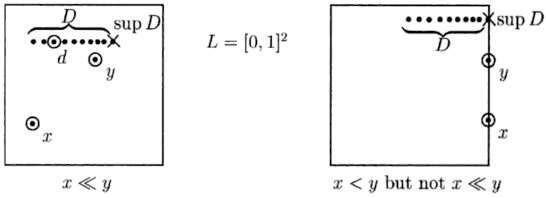
\includegraphics[scale=0.7]{figuurway.jpg}\\
  \caption{The ``Way Below''-relation on the lattice $[0,1]^2$.}\label{figuurway}
\end{figure}

\end{example}




\begin{theorem}
The direct product $\prod_{j \in J}L_j$ of a family pointed dcpo's is again a pointed dcpo with as way-below relation ($x, y \in \prod_{j \in J}L_j$):
$$x \ll y \Leftrightarrow x_j \ll y_j \;\forall j \in J \text{and } x_i = 0 \text{ for all but finitely many } i \in I$$
\end{theorem}

\begin{proof}
That being a dcpo is preserved under direct products is already proven in property \ref{directeproducten}, that each is preserves having a least element follows immediately from the definition of the pointwise order. Now, we prove the characterization of the way-below relation in such a direct product.  Suppose first that $x \ll y$, for every finite set $F \subseteq J$, define $y^F \in \prod_{j \in J}L_j$ as follows:
\begin{equation*}
  y_j^F=\begin{cases}
    y_j & \text{if $j \in F $}\\
    0 & \text{if $j \not\in F $}
  \end{cases}
\end{equation*}
Than $\{y^F | F \subset J \text{ finite}\}$ is directed and its supremum is $y$. As $x \ll y$, there is some finite subset $F \subseteq J$ such that $x \leq y^F$, whence $x_j = 0 \;\forall j \not\in F$.
In order to show that $x_j \ll y_j \;\forall j \in J$, fix $j$ and consider any directed set $D \subset L_j$ such that $y_j \leq \sup D$. To every $d \in D$ we associate the element $\overline{d} \in \prod_{j \in J}L_j$ defined by:
\begin{equation*}
  \overline{d}_i=\begin{cases}
    d & \text{if $i = j$}\\
    y_i & \text{if $i \neq j $}
  \end{cases}
\end{equation*}
The family $\{\overline{d}|d\in D\}$ is directed and $y \leq \sup_{d \in D}\overline{d}$. As $x \ll y$, there is some $d \in D$ such that $x \leq \overline{d}$, whence $x_j \leq d$.\\

For the converse, suppose that $x_j \ll y_j \;\forall j \in J$ and that there is a finite set $F \subset J$ such that $x_j = 0 \;\forall j \not\in F$. Let $D$ be any directed set in $\prod_{j \in J}L_j$ such that $y \leq \sup D$. Then $y_j \leq \sup_{d\in D}d_j$ for every $j \in J$. As $x_j \ll y_j$, for every $j \in J$, there is a $d^j \in D$ such that $x_j \leq d^j_j$ (= $j$th component of $d^j$). As $D$ is directed, there is a $d \in D$ such that $d^j \leq d \;\forall j \in F$. Thus $x_j \leq d_j \;\forall j \in F$. As $x_j = 0 \;\forall j \not\in F$, we conclude that $x \leq d$. This proves that $x \ll y$.

\end{proof}


\begin{example}
If $L$ is a complete chain, and we consider the partially ordered \emph{direct power} $L^I$ of $L$ in the pointwise ordering, then in the complete lattice $L^I$ we find $x \ll y$ iff $x_i \ll y_i$ for all $i \in I$ and $x_i = 0$ for all but a finite number of indices $i$. This immediately results from the previous theorem. When $I$ is infinite, this circumstance obviously justifies the ``way'' in ``way below".
\end{example}
\begin{example}
Consider a special case from the previous example, when $L$ is just the two element lattice and we can regard $L^I$ as the powerset lattice: in the powerset of $I$, the relation $A \ll B$ just means that $A$ is a finite subset of $B$.
\end{example}

\begin{example}\label{kutvoorbereiding}
Let $I$ a random set and $2^I$ be the powerset of $I$. We can also consider $2^I$ as the functions of $I$ to the set $\{0, 1\}$. In other words, $J \subseteq I$ can be written as
\begin{equation*}
  J = f: I \to \{0,1\}: j \mapsto \begin{cases}
    1 & \text{if $j \in A $}\\
    0 & \text{if $j \not\in A $}
  \end{cases}
\end{equation*}
Conversely, we can define $K$ as the function $y: I \to \{0, 1\}$. Let $A, B \subseteq I$ with $A \ll B$, then it follows from the previous example that $A$ is a finite subset of $B$.
\end{example}


\subsection{Domains}
\begin{definition}
A poset $L$ is called \emph{continuous} if $\downdownarrow x$ is directed with supremum $x$ for all $x \in L$.
\end{definition}

\begin{definition}
A dcpo which is continuous as a poset will be called a \emph{domain}.
\end{definition}


\begin{definition}
A subset $B$ of a dcpo $L$ is a \emph{basis} for $L$  if for all $x \in L, \downdownarrow x \cap B$ is directed with supremum $x$.
\end{definition}

\begin{lemma}
A dcpo $L$ is continuous iff it has a basis $B$.
\end{lemma}
\begin{proof}
If the dcpo $L$ is continuous take $B = L$. 

Conversely, if the dcpo $L$ has a basis $B$, take a random element $x \in L$, we must proof that every pair of elements in $\downdownarrow x$ has an upper bound. Take $y, z \in \downdownarrow x$,  because $\sup(\downdownarrow x \cap B) = x$, there must be elements $a, a' \in \downdownarrow x \cap B$ above $y, z$ (because, otherwise, $y$ or $z$ would be an upper bound of $\downdownarrow x \cap B$  smaller than $x$, contradicting the fact that $x$ is the supremum). Because $\downdownarrow x \cap B$ is directed, $a$ and $a'$ have an upper bound $w$ in $\downdownarrow x \cap B$, of course, $w$ is also in $\downdownarrow x$ and an upper bound of $y$ and $z$. 
 
 It's easy to see that $x$ is also the supremum of $\downdownarrow x$, because $\downdownarrow x \cap B$ has as supremum $x$ and the set $ \downdownarrow x$ will only contain elements `way below' $x$.
\end{proof}

\begin{definition}
A poset is \emph{algebraic} if its compact elements form a basis. A poset is \emph{$\omega$-continuous} if it has a countable basis.
\end{definition}

The notation $\int(S)$ is used to indicate the interior of a set $S$ and is defined as the set of all interior points of $S$, or, in other words, the largest  open set contained in $S$. This notation is used in the next example.

\begin{example} \textbf{(The Interval Domain)}
The collection of compact intervals of the real line:
$$\mathcal{C}(\R) = \{[a, b] | a, b \in \R \text{ and } a \leq b \}$$
ordered under reverse inclusion
$$[a, b] \leq [c, d] \Leftrightarrow [c, d] \subseteq [a, b]$$
is a \emph{$\omega$-continuous} dcpo ($\omega$-domain). The supremum of a directed set $S \subset \mathcal{C}(\R)$ is $\cap S$.

If we take a look at the way-below relation then we can proof the relation is characterized by $$[a, b] \ll [c, d] \Leftrightarrow [c, d] \subseteq ]a, b[.$$ 
Let's proof this characterization, consider first $[a, b] \ll [c, d]$. From property \ref{wayprop}(i) we know that $[c, d] \subseteq [a, b]$. The only thing left to prove is thus that neither $a$, nor $b$ is in $[c, d]$. Suppose the opposite: $a \in [c,d]$, this means $c = a$. Consider the set $I = \{[c-\epsilon, d] | \epsilon \geq 0 \}$, $I$ is directed with $\sup I = \bigcap I = [c, d]$. Hence there exists an $\epsilon' > 0$ wherefore $[c-\epsilon', d] \subseteq [a, b]$, a contradiction with $c = a$. With the same arguments, one can prove that also $b \not\in [c,d]$.

Conversely, suppose $[c, d] \subseteq ]a, b[$, take a directed subset $D \subseteq \mathcal{C}(\R)$, $\sup D = \cap D$, the relation $\cap D \subseteq [c, d] \subseteq [a,b]$ must imply the existence of $[d_x, d_y] \subseteq [a, b]$. Because $\cap D$ is the intersection of compact intervals, $\cap D$ is of the form $[y, z]$. So there must exist a $y_1$ with $y \geq y_1 \geq a$ such that $[y_1, z_1] \in D$ and there must exist a $z_2$ with $z \leq z_2 \leq b$ such that $[y_2, z_2] \in D$, because $D$ is directed $[y_1, z_1]$ and $[y_2, z_2]$ have an upper bound $[d_x, d_y]$ for which holds $[d_x, d_y] \subseteq [y_1, z_1]$ and $[d_x, d_y] \subseteq [y_2, z_2]$. Thus $[d_x, d_y] \subseteq [y_1, z_1]\cap [y_2, z_2]$. By construction  $[y_1, z_1]\cap [y_2, z_2]$ is a subset of $[a,b]$. It holds that $[d_x, d_y] \subseteq [a,b]$.

It follows that:
\begin{eqnarray*}
\downdownarrow [c, d] &= \{ [a, b] \subset \R | [a, b] \ll [c, d]  \} \\
&= \{ [a, b] \subset \R | [c, d] \subset ]a, b[  \}
\end{eqnarray*}
The set $\downdownarrow [c, d]$ has obviously $[c,d]$ as it's supremum. To show that $\downdownarrow [c, d]$ is directed, take two elements $[y_1, z_1], [y_2, z_2] \in \downdownarrow [c, d]$ and consider $I = [y_1 \vee y_2, z_1 \wedge z_2]$, $I$ is an element of $\downdownarrow [c, d]$ because $[c, d] \subset ]y_1, z_1[$ and $[c, d] \subset ]y_2, z_2[$ proves that $[c, d] \subset ]y_1, z_1[ \cap ]y_2, z_2[$ so $I = [y_1, z_1] \cap [y_2, z_2] \in \downdownarrow [c,d]$. Of course $I$ is an upper bound of $[y_1, z_1]$ and $[y_2, z_2]$, it is even their supremum. This proves that $\mathcal{C}(\R)$ is a domain.
\end{example}

\begin{example}\label{2Malg}
Let $M$ be a set and $L = 2^M$, the powerset of $M$, then $K(L)= \{F \subset M: F \text{ is finite}\}$ and $\downarrow X = \{F \subset M| F \subset X\}$. It follows that $\downarrow X \cap K(L) = \{F \subset X | F \text{ is finite}\}$. It's clear that $\sup(\downarrow X \cap K(L)) = X$. From example \ref{kutvoorbereiding} it follows that $\downdownarrow x = \downarrow x \cap K(L)$. The union of $\downarrow x \cap K(L)$ is clearly $x$ itself, thus $\sup \downdownarrow x = x$. It follows that $2^M$ is an algebraic continuous lattice.
\end{example}

\begin{theorem}
The direct product $\prod_{j\in J}L_j$ of a family  pointed domains $L_j, j \in J$ is itself a pointed domain with as way-below relation ($x, y \in \prod_{j \in J}L_j$):
$$x \ll y \Leftrightarrow x_j \ll y_j \;\forall j \in J \text{and } x_i = 0 \text{ for all but finitely many } i \in I$$
\end{theorem}

\begin{proof}
In property \ref{directeproducten} we already proved that the direct product of a family dcpo's is itself a dcpo for the pointwise ordering, so the only thing that is left to prove is that if every dcpo in such a family is continuous, the direct product is also continuous. Take an element $(x_j)_{j\in J} \in \prod_{j \in J}L_j$, for every $j \in J$ it holds that $\downdownarrow x_j$ is directed with supremum $x_j$, this means that $\downdownarrow(x_j)_{j\in J}$ is also directed with supremum $(x_j)_{j\in J}$, which proves continuity.
\end{proof}


\begin{lemma}\label{lemmavoor}
If $x \ll z$ and if $z \leq \sup D$ for a directed set $D$ in a continuous poset $L$, then $x \ll d$ for some element $d \in D$.
\end{lemma}

\begin{proof}
Let $D$ be a directed set with $z \leq \sup D$, and let $I = \cup\{\downdownarrow d | d \in D\}$. By continuity, $\sup I = \sup D$, so $x \ll z \leq \sup D = \sup I$. 

I is a directed lowerset. The must exist a $u \in I$ with $x \leq u$ (otherwise, $x$ is an upper bound of $I$ smaller than $z$ and thus smaller than $\sup I$, a contradiction). Because $u \in I$, there must exist a $d \in D$ such that $u \in \downdownarrow d$ for some $d \in D$, but this means that $u \ll d$. By property \ref{wayprop}(ii), we conclude that $x \ll d$.
\end{proof}

\begin{theorem}\label{interpolation}\textbf{(Interpolation property)} In a continuous posets L, the way-below relation satisfies the interpolation property $$x \ll z \Rightarrow \exists y: x \ll y \ll z.$$
\end{theorem}
\begin{proof}
This follows immediately from the previous lemma, by choosing $D = \downdownarrow z$ and recalling that $z = \sup \downdownarrow z$, by continuity of $L$.
\end{proof}

\section{Scott convergence}
In the introduction, we discussed the rich order theoretic structure of lattices, dcpo's and domains. We also introduced the way-below relation on these structures. The aim of this section is to introduce the Scott topology and its connection with convergence given in order theoretic terms by lower limits (or liminfs). Lower limits are defined of nets in dcpo's and will give meaning to the convergence of these nets. Starting from the set of convergent nets we will be able to construct a topology on dcpo's that became famous as the Scott topology  (named after the mathematician Dana Scott). In general topology this type of definition is common in associating open sets with a class of nets given as convergent. It isn't surprising that this definition of the Scott topology on a dcpo will characterize rather than exhibit open sets. When defining the Scott topology on domains, the convergence of nets will be topological which will characterize domains in a nice way.
\subsection{Lower semicontinuous functions}
\begin{definition}\label{semicontinuous}
Consider an extended real-valued function $f$ from a metric space $X$, $f: X \rightarrow \overline{R}$. It is \emph{lower semicontinuous} if and only if it satisfies any of the following equivalent conditions:
\begin{enumerate}
  \item for each real number $t$, the set $f^{-1}(]t, \infty])$ is open $X$;
  \item for any sequence $x_n$ converging to $x$ in $X$, the cluster points $c$ of the sequence $f(x_n)$ satisfy $f(x) \leq c$;
  \item for any sequence $x_n$ converging to $x$ in $X$, $f(x) \leq \liminf_n f(x_n)$, where $\liminf_n f(x_n) = \sup_n\inf_{m \geq n} f(x_m)$
\end{enumerate}

\end{definition}
In the above, sequences are adequate because $X$ is metric; in a more abstract setting nets would be required. Note that the range $\overline{R}$ is a complete continuous lattice. In order to treat the concepts emerging in the conditions (1), (2) and (3) in a systematic fashion, we describe on an arbitrary dcpo that structure of convergence (with its associated topology) which pertains precisely to the idea of lower semicontinuity. Evidently, the lower limit is a vital ingredient.

\subsection{$\mathcal{S}$-limits}

\begin{definition} \textbf{(Lower limit or liminf)} Let $L$ be a complete semilattice. For any net $(x_j)_{j\in J}$ we write
$$\liminf_j x_j = \sup_j \inf_{i \geq j} x_i,$$
and call $\liminf_j x_j$ the \emph{lower limit} or \emph{liminf} of the net.
\end{definition}

\begin{definition} \textbf{($\mathcal{S}$-limit)} Let $\mathcal{S}$ denote the class of the pairs $((x_j)_{j\in J}, x)$ such that $x \leq \liminf_j x_j$ ($\mathcal{S} = \{((x_j)_{j\in J}, x) | x \leq \liminf_j x_j \}$ . For each such pair we say that $x$ is an $\mathcal{S}-limit$ of $(x_j)_{j \in J}$ and we write briefly $x \equiv_{\mathcal{S}} \lim x_j$.
\end{definition}
If we generalize this definition to dcpo's, we have to take into consideration that a dcpo can lack an infinium for each directed subset. This give rise to the notion of an \emph{eventual lower bound}.

\begin{definition}\textbf{(Eventual lower bound)} Let $L$ be a dcpo. An element $y \in L$ is an \emph{eventual lower bound} of a net $(x_j)_{j\in J}$ in $L$ if there exists $k \in J$ such that $y \leq x_j$ for all $j \geq k$.
\end{definition}

An equivalent definition for the class $\mathcal{S}$ is defined as:

\begin{definition}
 Let $\mathcal{S}$ denote the class of the pairs $((x_j)_{j\in J}, x)$ such that $x \leq \sup D$ for some directed set $D$ of eventual lower bounds of the net $(x_j)_{j\in J}$. For each such pair we say again that $x$ is an $\mathcal{S}-limit$ of $(x_j)_{j \in J}$.
\end{definition}

\begin{definition}If the set of all eventual lower bounds of $(x_j)_{j\in J}$ has a supremum which is also a directed supremum of some subset off the set of eventual lower bounds (i.e. is an $\mathcal{S}$-limit of $(x_j)_{j\in J}$), then this supremum is called the \emph{lower limit} or the \emph{liminf} of the net, written $\liminf_j x_j$.
\end{definition}

The second definition of $\mathcal{S}$ and of the liminf for dcpo's, when applied to complete semilattices, agrees with the first definition of $\mathcal{S}$ and of the liminf for complete semilattices. Indeed if $\inf_{i \geq j}x_i$ exists for all $j \in J$, write $y_j = \inf_{i \geq j} x_i$. Then the collection $Y$ of all such $y_j$ is directed an the set of all eventual lower bounds is equal to $\downarrow Y$. Thus $\sup Y = \liminf_j x_j$.

\subsection{Convergence and topology}
We now use the general relation between \emph{convergence} and \emph{topology}. If on any set $L$ one is given an arbitrary class $\mathcal{L}$ of pairs $((x_j)_{j\in J}, x)$ consisting of a net and an element of $L$, then associated with $\mathcal{L}$ is a family of sets
$$\mathcal{O}(\mathcal{L}) = \{U \subseteq L | \text{ if } ((x_j)_{j\in J}, x) \in \mathcal{L} \text{ and } x \in U \text{ then eventually } x_j \in U\}.$$

\begin{property}
$\mathcal{O}(\mathcal{L})$ is a topology on $L$.
\end{property}
\begin{proof}
Clearly both $\emptyset$ and $L$ belong to $\mathcal{O}(\mathcal{L})$.

Take $A, B \in \mathcal{O}(\mathcal{L})$, let $((x_j)_{j\in J}, x) \in \mathcal{L}$ and $x \in A \cap B$, it follows that eventually $x_j \in A$ and eventually $x_j \in B$, in other words there exists elements $k_1, k_2 \in J$  such that for every $j \geq k_1$ it follows that $x_j \in A$ and for every $j \geq k_2$ it follows that $x_j \in B$. Take an upper bound $k$ of $k_1$ and $k_2$, than $\forall j \geq k: x_j \in A \cap B$. So $\mathcal{O}(\mathcal{L})$ is closed under the formation of finite intersections. A same argument can be used to proof that $\mathcal{O}(\mathcal{L})$ is also closed under the formation of arbitrary unions.
\end{proof}

By definition we know that, for any $((x_j)_{j\in J}, x) \in \mathcal{L}$, the element $x$ is a limit of the net $x_j$ relative to the topology $\mathcal{O}(\mathcal{L})$. Since however, $\emptyset$ and $L$ may very well be the only elements of $\mathcal{O}(\mathcal{L})$, what makes $\mathcal{O}(\mathcal{L})$ the indiscrete topology, we are obviously not saying very much; specific information information on $\mathcal{L}$ must become available before one can hope to get a close link between $\mathcal{L}$ and $\mathcal{O}(\mathcal{L})$. Fortunately, in our present situation, we do have specific information about our class $\mathcal{S}$. We begin exploiting it by characterizing the sets $U \in \mathcal{O}(\mathcal{S})$.

\begin{theorem}\label{scottprot} Let $L$ be dcpo and $U \subset L$. Then $U \in \mathcal{O}(\mathcal{S})$ iff the following two conditions are satisfied:
\begin{enumerate}[(i)]
    \item $U = \uparrow U$;
    \item $\sup D \in U$ implies $D \cap U \neq \emptyset$ for all directed set $D \subseteq L$.
\end{enumerate}
\end{theorem}
\begin{proof}
First, suppose $U \in \mathcal{O}(\mathcal{S})$. To prove (i), assume $u \in U$ and $u \leq x$. then $u \leq x = \liminf  x$ with the constant net $(x)$ with value $x$, so by definition $((x), u) \in \mathcal{S}$. Since we have that $u \in U \in \mathcal{O}(\mathcal{S})$, we conclude from the definition of $\mathcal{O}(\mathcal{S})$ that the net $(x)$ must be eventually in $U$. This means $x \in U$. So $U = \uparrow U$.

In order to prove (ii), let $D$ be a directed set in $L$ with $\sup D \in U$. Consider the net $(x_d)_{d \in D}$ with $x_d = d$. Now $inf_{c\geq d} x_c = d$, and thus $\liminf_{d \in D} x_d = \sup D \in U \in \mathcal{O}(\mathcal{S})$. Since $((x_d)_{d \in D}, \sup D) \in \mathcal{S}$, we conclude that $d = x_d$ is eventually in $U$; whence $D \cap U \neq \emptyset$.\\

Second, suppose that $U$ satisfies (i) and (ii). We take $((x_j)_{j \in J}, x) \in \mathcal{S}$ with $x \in U$, and we must show that $x_j$ is eventually in $U$. By the definition of $\mathcal{S}$, we have $x \leq \sup D$ for some directed set $D$ of eventual lower bounds of $(x_j)_{j \in J}$. Then $x \in U$ implies $\sup D \in U$ by (i), and then $d \in U$ for some $d \in D$ by (ii). By definition $d \leq x_i$, for all $i \geq j$ for some $j \in J$. Again by (i), $x_i \in U$ for all $i \geq j$. Thus $U \in \mathcal{O}(\mathcal{S})$.
\end{proof}

\begin{definition}\textbf{(Scott topology)} A subset $U$ of a dcpo $L$ is called \emph{Scott open} iff it satisfies the conditions of the previous theorem. The complement of a Scott open set is called \emph{Scott closed}. The collection of all Scott open subset of $L$ will be called the \emph{Scott topology} of L and will be denoted by $\sigma(L)$.
\end{definition}

\begin{definition}\textbf{($\mathcal{S}$-property)}
We say that a subset $X$ of a dcpo $L$ has the $\mathcal{S}$-property if the following condition is satisfied:\\
 
 $\sup D \in X$ for any directed set $D$, then there is an $y \in D$ such that $x \in X$ $\forall x \in D$ with $x \geq y.$
\end{definition}

\begin{theorem}\label{lijstdcpo} If any dcpo L we have the following properties:
\begin{enumerate}[(i)]
    \item a set is Scott closed iff it is a lower set closed under directed sups,
    \item $\downarrow x = \overline{\{x\}}$ (closure with respect to $\sigma(L)$) for all $x \in L$,
    \item $\sigma(L)$ is a $T_0$ space,
    \item every upper set is the intersection of its Scott open neighborhoods,
    \item a set is Scott open iff it is an upper set satisfying the $\mathcal{S}$-property,
    \item every lower set has the $\mathcal{S}$-property,
    \item the collection of all subsets having the $\mathcal{S}$-property is a topology.
\end{enumerate}
\end{theorem}

\begin{proof}
\begin{enumerate}[(i)]
    \item $A \subseteq L$ is a lower set iff $L \setminus A$ is an upper set, and $L \setminus A$ satisfies the second condition in Theorem \ref{scottprot} iff $A$ closed under directed sups.
    \item We have that $\downarrow x$ is the smallest lower set containing $x$, and it happens to be closed under directed sups. It follows from (i) that $\downarrow x$ is the smallest Scott closed set that contains $x$.
    \item If $\overline{\{x\}} = \overline{\{y\}}$, then $\downarrow x = \downarrow y$ by (ii); thus $x = y$, which proves that $\sigma(L)$ is a $T_0$-space.
    \item Every upper set $B$ is the intersection of the sets $L \setminus \downarrow x$ where $x \in L \setminus B$ ($B = \cap_{x \in L \setminus B} L \setminus \downarrow x$). When applying (ii), these sets are Scott open.
    \item This follows immediately from the second condition in Theorem \ref{scottprot}.
    \item Let $X$ be a lower set, $D$ a directed subset of $L$ with $\sup D \in X$ then it holds for all $d \in D$ that $d \leq \sup D$ which means that $d \in X = \downarrow X$.
    \item First, $\emptyset$ and $L$ satisfy the $\mathcal{S}$-property. Let us now prove that the $\mathcal{S}$-property stays satisfied under the formation of finite intersections of sets with the $\mathcal{S}$-property. Take the sets $A, B \subseteq L$ which satisfy the $\mathcal{S}$-property, and take $D \subseteq L$ a directed subset of $L$ with $\sup D \in A \cap B$. Of course $\sup D \in A$ and $\sup D \in B$, so there exists elements $y_1, y_2 \in D$ such that $\forall x \geq y_1$ it follows that $x \in A$ and $\forall x \geq y_2$ it follows that $x \in B$. Let $y$ be an upper bound of $y_1$ and $y_2$, then it holds for all $x \in D$ with $x \geq y$ that $x \in A \cap B$. The fact that the $\mathcal{S}$-property is also satisfied under the formation of arbitrary unions of sets with the $\mathcal{S}$-property is provable in the same way.
\end{enumerate}
\end{proof}
\begin{example}\label{unitkut}
If $L$ is the unit interval: $L = [0,1]$, then $L$ is a complete chain, hence a dcpo.  Any Scott open set has the form $]x,1]$ if $0 \leq x \leq 1$ or $[0, 1]$. $]x, 1]$ is Scott open by the second condition of the previous theorem because $]x, 1] = \uparrow x \setminus \{x\} = L \setminus \downarrow x$. $[0,1]$ is Scott open because it's an upper set that satisfies trivially the $\mathcal{S}$-property.

Conversely, let $U$ be a Scott open set then it follows from the first condition from Theorem \ref{scottprot} that $U = \uparrow U$, this means that $U$ can be $]x, 1]$ or $[x, 1]$. But consider $D = L \setminus [x, 1]$ with $x \neq 0$, $D$ is clearly a directed set with $\sup D = x \in U$ but $U \cap D = \emptyset$ so $[x, 1]$ with $x \neq 0$ doesn't satisfy the conditions to be Scott open. The only Scott open sets are thus $]x, 1]$ with $0 \leq x \leq 1$ together with $L$.
\end{example}


\begin{example}
On the chain $L = \{0, 1\}$, the Scott topology equals the Sierpinski topology, $\sigma(L) = \{\emptyset, \{1\}, L\}$.
\end{example}

\begin{theorem}\label{begindomein}
If $L$ is a domain, then all sets $\upuparrow x$ for $x \in L$ are Scott open. Conversely, if $L$ is a dcpo and $y \in \int(\uparrow x)$, then $x \ll y$.
\end{theorem}

\begin{proof}
Let $D$ be a directed set with $\sup D \in \upuparrow x$, then Lemma \ref{lemmavoor} implies the existence of a $d \in D$ such that $x \ll d$ en thus $d \in \upuparrow x$. Hence $\upuparrow x$ is Scott open by definition.

Suppose $L$ is a dcpo and $y \in \int(\uparrow x)$, if $D$ is a directed set with $y \leq \sup D$, then $\sup D \in \int(\uparrow x)$ because $\int(\uparrow x)$ is Scott open and $x \leq d \leq \sup D$. It follows that $D \cap \int(\uparrow x) \neq \emptyset$. Hence, there exists a $d \in D$ with $d \in \int(\uparrow x)$, thus $x \leq d$ and it follows that $x \ll y$.
\end{proof}
\begin{remark}
From the previous theorem we conclude that, when $L$ is a domain, for each $x \in L$ it holds that $\int(\uparrow x) = \upuparrow x$.
\end{remark}
In order to conclude this section, we must return to the discussion of the concept of convergence and investigate whether the Scott topology (which we derived from a convergence concept) is in fact adequate to describe in topological terms the $\mathcal{S}$-convergence.

\begin{definition}\textbf{(Topological)}If $\mathcal{S}$ is precisely the class of convergent nets for the Scott topology, then we say that $\mathcal{S}$ is \emph{topological}.
\end{definition}

\begin{theorem}
Let $L$ be a domain. Then $x \equiv_{\mathcal{S}} \lim x_j$ iff the net $(x_j)_{j\in J} \rightarrow x$ with respect to the Scott topology $\sigma(L)$. In particular, the $\mathcal{S}$-convergence is topological.
\end{theorem}
\begin{proof}
By definition of the Scott topology, if $x \equiv_{\mathcal{S}} \lim x_j$, then $(x_j)_{j\in J} \rightarrow x$ with respect to $\sigma(L)$.

Conversely, suppose that we have a convergent net $(x_j)_{j\in J} \rightarrow x$ in the Scott topology. For each $y \in \downdownarrow x$, we have that $\upuparrow y$ is a Scott open set containing $x$ by Theorem \ref{begindomein}. Thus the net $(x_j)_{j\in J}$ is eventually in $\upuparrow y$, and hence $y$ is an eventual lower bound for the net. Since $\downdownarrow x$ is directed and has supremum $x$, we have $((x_j)_{j\in J}, x) \in \mathcal{S}$.
\end{proof}
If the $\mathcal{S}$-convergence is topological in a dcpo, the dcpo is a domain, thus the converse is also true:
\begin{lemma}
Let L be a dcpo, if the $\mathcal{S}$-convergence is topological, then $L$ is a domain.
\end{lemma}

\begin{proof}
By Lemma \ref{scottprot} the topology arising from $\mathcal{S}$-convergence, is the Scott topology. Thus if $\mathcal{S}$-convergence is topological, we must have $x \equiv_{\mathcal{S}} \lim x_j$ iff the net $(x_j)_{j\in J} \rightarrow x$ with respect to $\sigma(L)$. Let $x \in L$. Define $$I = \{(U,n,a) \in \mathcal{N}(x) \times \N \times L | a \in U\},$$
where $\mathcal{N}(x)$ consists of all Scott open sets containing $x$, and define an order on $I$ to be the lexicographic order on the first two coordinates, that is, $(U, m, a) < (V, n, b)$ iff $V$ is a proper subset of $U$ or $U = V$ and $m < n$. Let $x_i = a$ for $i = (U, n, a) \in I$ define the net. Then it is easy to see that $(x_i)_{i \in I}$ converges to $x$ in the Scott topology. Thus $x \equiv_\mathcal{S} \lim x_i$, and we conclude that there exists a directed set $D$ of eventual lower bounds of $(x_i)_{i\in I}$ such that $x \leq \sup D$. Let $d \in D$. Then there exists $i = (U, m, a) \in I$ such that $(V, n, b) = j \geq i$ implies $d \leq b$. In particular, we have $(U, m + 1, b) > (U, m, a)$ for all $b \in U$, and thus $d$ is a lower bound for $U$, i.e., $x \in \int(\uparrow d)$. By Theorem \ref{begindomein}, $d \ll x$. Since $D$ is directed with supremum greater than or equal to $x$, we conclude that $x$ is the directed supremum of $D \subseteq \downdownarrow x$. Since $x$ was arbitrary, we conclude that $L$ is a domain.
\end{proof}

\subsection{The Scott topology of domains}
So now we know that for a dcpo $L$, that $L$ being a domain is equivalent with saying that the $\mathcal{S}$-convergence is topological for the Scott topology $\sigma(L)$. This means that domains are extremely useful to study lower semicontinuity completely in topological terms (see below in section 3).

\begin{theorem}\label{domeinkak}
Let $L$ be a domain
    \begin{enumerate}[(i)]
        \item An upper set $U$ is Scott open iff for every $x \in U$ there is a $u \in U$ such that $u \ll x$.
        \item The sets of the form $\upuparrow x$, $x \in L$, form a basis for the Scott topology. In particular, each point $x \in L$ has a $\sigma(L)$ neighborhood basis consisting of the sets $\upuparrow x$ with $u \ll x$.
        \item With respect to $\sigma(L)$, we have $\int(\uparrow x) = \upuparrow x$.
        \item With respect to $\sigma(L)$, we have for any subset $X \subseteq L$
        $$\int(X) = \displaystyle\bigcup{\{\upuparrow u \; | \upuparrow u \subseteq X\}}$$.
    \end{enumerate}
\end{theorem}
\begin{proof}
\begin{enumerate}[(i)]
        \item Let $U$ be Scott open and $x \in U$. As in a domain the set $\downdownarrow x$ is directed and has supremum $x$, we conclude that there is a $u \ll x$ with $u \in U$ by the second condition of Lemma \ref{scottprot}.

            If conversely for every $x \in U$ there is a $u \in U$ such that $u \ll x$ then $U$ is the union of the sets $\upuparrow u$, $u \in U$, which are Scott open by Theorem \ref{begindomein}; hence, $U$ is Scott open.
        \item Follows immediately of (i).
        \item If $y \in \int(\uparrow x)$, then by (i) there is a $u \in \uparrow x$ with $u \ll y$. But then $y \in \upuparrow x$. Obviously $\upuparrow x \subseteq \int(\uparrow x)$.
        \item Follows immediately of (ii).
    \end{enumerate}
\end{proof}
\begin{example}
\begin{figure}
  \centering
  % Requires \usepackage{graphicx}
  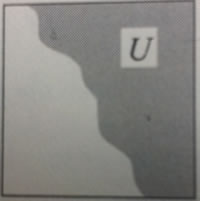
\includegraphics[scale=0.6]{scottopen.jpg}\\
  \caption{The Scott open sets in the square $L = [0, 1]^2$.}\label{scottplane}
\end{figure}

Let $L = [0, 1]^2$, the square with the pointwise ordering, which is of course a domain because it's a continuous lattice. From the example \ref{unitkut}, we know that $\sigma([0,1]) = \{]x, 1] | 0 \leq x \leq 1 \} \cup \{[0,1]\}$. An interesting question is now: is the product topology on L generated by the rectangles $]x_1, 1] \times ]x_2, 1]$ (with $x_1, x_2 \in [0, 1])$ is also the Scott topology on $L$? Indeed, by the previous theorem $\sigma(L)$ has a basis $\{\upuparrow x | x \in L\}$. Take an element $(x_1, x_2) \in L$, then the set $\upuparrow (x_1,x_2)$ consist of all the points ``way above'' ($\gg$) $x$, by example \ref{gewonelijn} we conclude that the collection of all these points are just the open rectangles. Thus the product topology indeed induces the Scott topology. Figure \ref{scottplane} shows a picture of these open sets.

We can also construct the Scott topology on $L = [0,1]^2$ in a different manner, in this construction a subset $U$ is Scott open iff it is an upper set and its open in the ordinary topology induced by the plane.  That $\sigma(L)$ is a subset of the ordinary topology is trivial, because $\upuparrow x$ is an element of the ordinary topology. Conversely, let $\uparrow V$ = $V$ and $V$ is an open set in the ordinary topology, now we have to proof that $V$ is also Scott open. Take an element $x \in V$, because $V$ is open for the ordinary topology it has an infinum $a$, namely the left corner such that $a \ll v$. By the previous theorem, $V$ is also Scott open.   So we see that in this topology every Scott open set of $[0,1]^2$ is the union of open upper rectangles. Note that these rectangles are the intersection of two sets of the form $L\setminus \downarrow x$.
\end{example}

\begin{theorem}\label{toevoeging}
If  $L$ is an algebraic domain then the Scott topology has a basis of sets $\uparrow k$ where $k \in K(L)$;

\begin{proof}
Let $U$ be a Scott open neighborhood of $x$. We recall that $x = \sup(\downarrow x \cap K(L))$ and $\downarrow x \cap K(L)$ is directed. By theorem \ref{scottprot}(ii), we find a $k \in \downarrow x \cap K(L) \cap U$. Then $\uparrow k = \upuparrow k$  ($k$ is compact, thus $k \ll k$, thus for a $y \in \uparrow k$, it follows that $k \ll y$) is a Scott open neighborhood of $k$, hence of $x$, with $\uparrow k \subseteq U$.
\end{proof}
\end{theorem}
\section{Scott-Continuous Functions}
By looking at the definition of the Scott topology on a dcpo, we automatically get a notion of continuity. We will define Scott-continuous maps as the maps preserving directed sups. 

\subsection{Definition}
\begin{theorem} For a function $f: S \rightarrow T$, with $S,T$ dcpo's, the following conditions are equivalent:
\begin{enumerate}
    \item $f$ is continuous with respect to the Scott topologies, that is $$f^{-1}(U) \in \sigma(S),\; \forall U \in \sigma(T),$$
    \item f preserves suprema of directed sets, that is, $f$ is order preserving and $f(\sup D) = \sup f(D)$, for all directed subsets $D$ of $S$,
    \item $f$ is order preserving and $f(\liminf_{j\in J} x_j) \leq \liminf_{j \in J} f(x_j)$, for any net $(x_j)_{j \in J}$ on $S$ such that $\liminf_{j\in J} f(x_j)$ both exists (this is of course always the case if $S$ and $T$ are complete semilattices).
    \item If $S$ and $T$ are domains, then $y \ll f(x)$ iff for some $w \ll x$ one has $y \ll f(w)$, for all $x \in S$ and $y \in T$.
    \item If $S$ and $T$ are domains, then $f(x) = \sup\{f(w)| w \ll x\},\;\forall x \in S.$
    \item If $S$ and $T$ are algebraic domains, then $k \leq f(x)$ iff for some $j \leq x$ with $j \in K(S)$ one has $k \leq f(j)$, for all $x \in S$ and $k \in K(T)$;
    \item If $S$ and $T$ are algebraic domains, $f(x) = \sup\{f(j) | j \leq x \text { and } j \in K(S),\; \forall x \in S\}$.
\end{enumerate}
\end{theorem}
\begin{proof}
(1)$\Rightarrow$(2): First we show that (1) implies that $f$ is order preserving: Suppose that $f(x) \not\neq f(y))$, then the Scott open set $V = T\setminus \downarrow f(y)$ contains $f(x)$. Thus $U = f^{-1}(V)$ is a Scott open neighborhood of $x$ by (1) not containing $y$. But then $x \not\neq y$ as $U$ is an upper set. Thus $x \neq y$ implies $f(x) \neq f(y)$.

Now let $D$ be a directed subset of $S$. Then $f(D)$ is directed and $\sup f(D) \neq f(\sup D)$, since $f$ is order preserving. Set $x = \sup D$ and $t = \sup f(D)$. We claim $f(x) \neq t$; Suppose $f(x) \not\neq t$. The Scott open set $T\setminus \downarrow t$ contains $f(x)$; thus, the inverse image $U = f^{-1}(T\setminus \downarrow t)$ is a Scott open neighborhood of $x$ in $S$ by (1). It follows that there is a $d \in D$ such that $d \in U$. Then $f(d) \in T\setminus \downarrow t$, that is, $f(d) \not \neq t = \sup f(D)$. This contradiction proves our claim.

(2)$\Rightarrow$(1): Let $A$ be a Scott closed subset of $T$. In order to show that $f^{-1}(A)$ is Scott closed in $S$ we take a directed subset $D$ of $f^{-1}(A)$. Then by (2) $f(\sup D) = \sup f(D)$. But $\sup f(D) \in A$ by Theorem \ref{lijstdcpo}(i), since $A$ is Scott closed and $f(D)$ is directed owing to the monotonicity of $f$. then $f(\sup D) \in A$, and hence $\sup D \in f^{-1}(A)$. Thus $f^{-1}(A)$ is Scott closed by the same theorem.

(3)$\Rightarrow$(2): Let $D$ be a directed set in $S$. If we define a set $(x_d)_{d\in D}$ and we set $x_d = d, d \in D$, then $\downarrow D$ is the set of all eventual lower bounds. Because $D \subset \downarrow D$ and $\sup D = \sup \downarrow D$ it follows that $\liminf_{d\in D} x_d = \sup D$, and, as $f(D)$ is directed by the monotonicity of $f$, similarly $\liminf f(x_d) = \sup f(D)$. Thus (3) implies $f(\sup D) \leq \sup f(D)$. As the converse inequality is true by the monotonicity of $f$, we deduce $f(\sup D) = \sup f(D)$.

(2)$\Rightarrow$(3): Suppose that $x = \liminf_j x_j$ for a net $(x_j)_{j \in J}$ in $S$ and $y = \liminf_j f(x_j)$, then there is a directed set $D$ of eventual lower bounds of the net $(x_j)_{j \in J}$ such that $x = \liminf_j x_j = \sup D$. By the monotonicity of $f$, every $f(d)$, $d \in D$, is an eventual lower bound of the net $(f(x_j))_{j \in J}$ and the set $f(D)$ is directed, whence $\sup f(D) \leq \lim_j f(x_j) = y$. From (2) we conclude $\liminf_j x_j = f(\sup D) = \sup f(D) \leq \liminf_j f(x_j)$.

From now on we assume that $S$ and $T$ are domains.

(2)$\Rightarrow$(5): Trivial, since $\downdownarrow x$ is directed and $x = \downdownarrow x$ (because $S$ is a domain). From (2) we can conclude that $f(x) = f(\sup \downdownarrow x) \leq \sup f(\downdownarrow x).$

(5)$\Rightarrow$(4): From (5) we can conclude that $f$ is monotone. Indeed, if $x \leq y$, then $\downdownarrow x \subseteq \downdownarrow y$ and consequently $f(x) = \sup f(\downdownarrow x) \leq \sup f(\downdownarrow y) = f(y)$. Now let $y \ll f(x) = \sup f(\downdownarrow x)$; since $f$ is monotone, $f(\downdownarrow x)$ is directed. Thus by Lemma \ref{lemmavoor}, there is a $w \ll x$ with $y \ll f(w)$. Conversely, if $y \ll f(w)$ for some $w \ll x$, then $y \ll f(x)$ by monotonicity of $f$ that $y \ll f(w) \ll f(x)$.

(4)$\Rightarrow$(1): Let $U \in \sigma(T)$ and $x \in f^{-1}(U)$. By Theorem \ref{domeinkak} there is a $y \in U$ with $y \ll f(x)$. By (4) we find a $w \ll x$ such that $y \ll f(w)$ we will have finished the proof if we show that $f(\upuparrow w) \subseteq U$. Now, take a $z$ with $w \ll z$. For every $y' \ll f(w)$ we have $y' \ll f(z)$ by (4); and consequently $f(w) = \sup \downdownarrow f(w) \leq f(z)$. But then $y \leq f(w)$ and $y \in U$, hence, $f(z) \in U$.

Now let $S$ and $T$ be algebraic domains.

Note that in an algebraic domain we have $x \ll y$ iff there is a compact element $k$ with $x \leq k \leq y$. Thus the equivalences (4) iff (6) and (5) iff (7) follow easily.
\end{proof}
\begin{definition}\textbf{(Scott-continuous)}
A function $f: S \rightarrow T$ between dcpo's is \emph{Scott-continuous} iff it satisfies the equivalent conditions in the previous theorem.
\end{definition}
\begin{example}
The identity map id$_X: X \rightarrow X$ on a dcpo $X$, defined by id$_X(x) = x$, for every $x \in X$, is always Scott continuous. Indeed, the inverse of every open set $U$ in $\sigma(X)$ is $U$ itself and thus the inverse is open.
\end{example}


\begin{example}
Every map preserving arbitrary sups is Scott-continuous. This follows easily from the second equivalent condition in the previous theorem.
\end{example}

\begin{example}
A function $f: X \rightarrow \overline{R}$, from a topological space into the extended set of reals is lower semicontinuous iff it is continuous with respect to the Scott topology on $\overline{R}$.
\end{example}

\subsection{Kleene Fixed-Point theorem}
The following fixed-point theorem for Scott-continuous self-maps on dcpo's is extremely useful. It was found by the American mathematician Stephen Cole Kleene and is therefore sometimes called the Kleene Fixed-Point theorem. One may notice that we dot need the full strength of directed completeness and Scott continuity here, but only $\omega$-completeness and $\omega$-continuity by which we mean that $\sup x_n$ exists and $f(\sup_n x_n) = \sup_n f(x_n)$ for all increasing sequences $x_0 \leq x_1 \leq x_2 \leq ...$.

\begin{theorem}\textbf{(Kleene Fixed-Point theorem)} Let $L$ be a dcpo with a least element $\bot$, then it has the following properties:
\begin{enumerate}[(i)]
  \item \textbf{Existence}: Every Scott-continuous self-map $f: L \rightarrow L$ has a least fixed-point, notated by \LFP($f$).
  \item \textbf{Construction}: The least fixed-point can be approximated by the recursively defined \emph{Kleene chain}:
      $$x_0 = \bot, \; x_{n+1} = f(x_n) = f^{n+1}(\bot)$$
      in the sense that
      $$\text{\LFP}(f) = \sup_n x_n = \sup_n f^n(\bot).$$
  \item \textbf{Preservation} Let $M$ be a second dcpo with bottom and let
 \begin{center}
  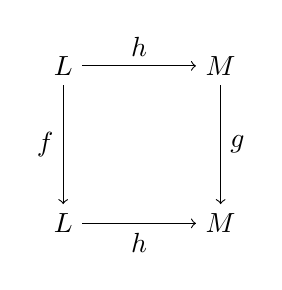
\begin{tikzpicture}[node distance=2cm, auto]
  \node (L) {$L$};
  \node (M) [right of=L] {$M$};
  \node (L2) [below of=L] {$L$};
  \node (M2) [right of=L2] {$M$};
  \draw[->] (L) to node {$h$} (M);
  \draw[->] (L) to node [swap] {$f$} (L2);
  \draw[->] (L2) to node [swap] {$h$} (M2);
  \draw[->] (M) to node {$g$} (M2);
\end{tikzpicture}
 \end{center}
 be a commuting diagram of Scott-continuous maps. Then
 $$h(\LFP(f)) = \LFP(g | \uparrow h(\bot)).$$
 If h is strict, i.e. if $h(\bot) = \bot$, the
 $$h(\LFP(f)) = \LFP(g).$$
\end{enumerate}
\end{theorem}
\begin{proof}
As $x_0 = \bot \leq f(\bot) = x_1$ and as $f$ is order preserving, we conclude that $x_1 = f(x_0)  \leq f(x_1) = x_2$, and by induction that $f(x_n) \leq f(x_{n+1})$ for all $n$. As the sequence $(x_n)$ is increasing, it has a least upper bound $x = \sup_n x_n$ in $L$. By the continuity of $f$, we have $f(x) = f(\sup_n x_n) = \sup_n f(x_n) = \sup_n x_{n + 1} = x.$ Thus $x$ is a fixed-point of $f$. It is the smallest fixed-point of $f$. Indeed, let $y = f(y)$ be another fixed-point, as $x_0 = \bot \leq y$, we get $x_1 = f(\bot) \leq f(y) = y$ and, by induction, $x_n \leq y$ for all $n$, whence $x = \sup_n x_n \leq y$. This proves (i) and (ii). For (iii) we first remark that $\uparrow h(\bot)$ is a dcpo with a smallest element $h(\bot)$ and that $g$ maps $\uparrow h(\bot)$ into itself, as $x \geq h(\bot)$ implies $g(x) = gh(\bot) = hf(\bot) \geq h(\bot)$. Hence the restriction of $g$ to $\uparrow h(\bot)$ has a least fixed-point and
\begin{align*}
h(\LFP(f)) &= h(\sup_n f^n(\bot))& &\text{by (ii)}\\
&= \sup_n hf^n(\bot)& &\text{as $h$ is Scott-continuous}\\
&= \sup_n g^nh(\bot)&   &\text{as the above diagram commutes}\\
&= \LFP(g | \uparrow h(\bot))&  &\text{by (ii).}
\end{align*}
\end{proof}

\begin{example}
The Kleene Fixed Point Theorem is essential in denotational semantics, where it is used to give meaning to recursive function definitions in programming languages. For example, the definition of factorial as the fucntion that maps $n \in \N$ to \texttt{f(n) = if $n$ = 0 then 1 else n.$f(n-1)$} is obtained as the least fixed point of the higher-order function $F$, mapping any function $f$ to the function $f'$ defined by \texttt{f($n$) = if $n$ = 0 then 1 else n.$f($n$-1)$}
\end{example}

\section{Categorical conclusion: Injective spaces}
In this final section, we'll use some category theory to search for topological spaces that we can become by considering the Scott topology on a continuous lattice. We'll proof a categorical relation between the injective $T_0$ spaces and the continuous lattices.

\begin{definition}
The category whose objects are dcpos and whose morphisms are Scott-continuous maps will be denoted by \emph{DCPO}, and the full subcategory of complete lattices by \emph{UPS}. The full subcategories of domains and continuous lattices are called \emph{DOM} and \emph{CONT} respectively. The full subcategories of algebraic domains and algebraic lattices are called \emph{ALGDOM} and \emph{ALG} respectively.
\end{definition}

\begin{definition}
Let $L$ be a continuous lattice, we call $\Sigma: CONT \rightarrow TOP$ the functor who associates $L$ with his Scott topology $\Sigma(L)$.
\end{definition}

\begin{definition}\textbf{(Injective space)}
A $T_0$-space $Z$ is called \emph{injective} iff every continuous map $f: X \rightarrow Z$ extends continuously to any space $Y$ containing $X$ as a subspace.
 \begin{center}
  \begin{tikzpicture}[node distance=2cm, auto]
  \node (Z) {$Z$};
  \node (X) [below of=Z] {$X$};
  \node (Y) [right of=X] {$Y$};
  \draw[->] (X) to node {$f$} (Z);
  \draw[>=latex,>->] (X) to node [swap] {j} (Y);
  \draw[->, dashed] (Y) to node [swap] {$f^*$} (Z);
\end{tikzpicture}
 \end{center}
\end{definition}
\begin{definition}\textbf{(Retract)}
Let $f: X\to Y, g: Y\to X$ be continuous functions whose composition $f\circ g: Y \to Y$ is the identity function on Y, then $f$ is a \emph{retraction} of $g$. $Y$ is called a \emph{retract} of \emph{X}.
\end{definition}
\begin{lemma}\label{karlakak}
\begin{enumerate}[(i)]
  \item Products of injective spaces are injective spaces.
  \item Retracts of injective spaces are injective spaces.
  \item If $Z$ is an injective space and $j: Z \to Y$ is a monomorphism, then $Z$ is a retract of $Y$.
\end{enumerate}
\end{lemma}
\begin{proof}\label{commproof}For (i), let $f$ space be a continuous function $f: X \to \prod_{i\in I}Z_i$, we have to show that this function extends continuously to any space $Y$ containing $X$ as a subspace. Let $p_i: prod_{i\in I}Z_i \to Z_i$, the i'th projection. Consider $f_i = p_i \circ f$ this a function from $X$ to $Z_i$ and thus it extends continuously to any space $Y$ containing $X$ as a subspace as $f_i^*$. Let $f^* = (f_i^*)_{i\in I}$, then $f^*$ is a continuous extension of $f$ to $Y$.

  \begin{center}
  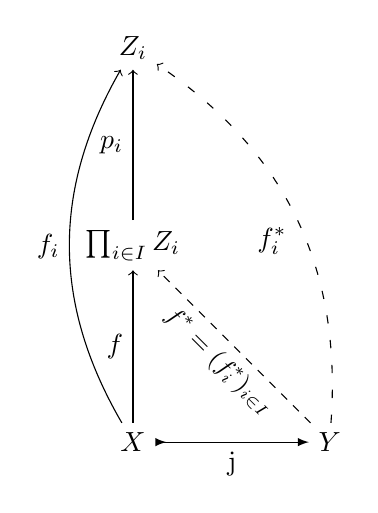
\begin{tikzpicture}[node distance=2.5cm, auto]
  \node (Z) {$\prod_{i\in I} Z_i$};
  \node (X) [below of=Z] {$X$};
  \node (Y) [right of=X] {$Y$};
  \node (A) [above of=Z] {$Z_i$};
  \draw[->] (X) to node {$f$} (Z);
  \draw[>=latex,>->] (X) to node [swap] {j} (Y);
  \draw[->, bend left] (X) to node {$f_i$} (A);
  \draw[->, bend right, loosely dashed] (Y) to node {$f_i^*$} (A);
  \draw[->] (Z) to node {$p_i$} (A);
  \draw[->, dashed] (Y) to node  [below,sloped]{\small{$f^* = (f_i^*)_{i\in I}$}} (Z);  
  
\end{tikzpicture}
\end{center}
For (ii), let $p: W \to Z$ be a retraction, so there exists a function $q: Z\to W$ such that $ p\circ q: \text{id}_Z$.  Let $W$ be an injective space, let $f: X \to Z$ be a continuous function and let $X$ be a subset of $Y$. It's clear that $q \circ f$ is continuous as composition of two continuous functions, the function goes from $X$ to $W$, so there exists a continuous extension $(q\circ f)^*: Y \to W$. It follows that $p\circ(q\circ f)^*$ is the continuous extension $f^*.$. Indeed, $p\circ(q\circ f)^*$ is continuous as composition of continuous functions and 
\begin{align*}
(p \circ(q \circ f)^*)|_X &=  p \circ(q \circ f)^*|_X
& = p \circ q \circ f
& = \text{id}_z \circ f
& = f
\end{align*}
For (iii), this is easy to prove when looking at the identity: $\text{id}_z: Z \to Z$ is a continuous function. Because $Z$ is an (injective) subspace of $Y$, there exists a continously extension $\text{id}_z^*$. It follows that $\text{id}_z \circ \text{id}_z^* = \text{id}_z$.
\end{proof}

\begin{example}The Sierpinski space, denoted by $\Sigma 2$, is injective. Indeed, suppose that $X$ is a subspace of $Y$ and that $f: X \to \Sigma 2$ is a continuous map. then $U = f^{-1}(1)$ is open in $X$ since $\{1\} \in \Sigma 2$. By the definition of the induced topology on $X$, there is an open set $V$ on $Y$ with $U = V \cap X$. Define $g: Y \to \Sigma 2$ so that $g^{-1}(1) = V$; it is continuous, and clearly $g|_X = f$.
\end{example}

\begin{lemma}\label{overbodigheidgehoopt}
\begin{enumerate}[(i)]
  \item For every set $M$ we have $\Sigma(2^M) = (\Sigma 2)^M$; thus: the Scott topology on $2^M$ and the product topology agree. Moreover, $\Sigma(2^M)$ is injective.
  \item Every $T_0$-space $X$ is embedded in some $(\Sigma 2)^M$.
  \item Every injective $T_0$-space $X$ is a retract of some $(\Sigma 2)^M$; that is, there is a continuous $f: (\Sigma 2)^M \to (\Sigma 2)^M$ with $f^2 = f$ and $\text{im} f$ homeomorphic to $X$
\end{enumerate}

\end{lemma}
\begin{proof}
\begin{enumerate}[(i)]
\item As $2^M$ is an algebraic lattice by example \ref{2Malg}, by theorem \ref{toevoeging} we now that $\Sigma(2^M)$ has as a basis for its topology the sets of the form $\uparrow$ where $k$ is compact in $2^M$. But by example \ref{kutvoorbereiding} we can consider every $k$ as a function from $M$ to $\{0, 1\}$ that takes on the value 1 only finitely often. The set $\uparrow k$, then, is exactly the class of functions that take the value 1 at least at the places that $k$ does.

Turning now to the product space $(\Sigma 2)^M$, we remark that, because $\{1\}$ is the only nontrivial open set of $\Sigma 2$, a basis for the open sets is given by putting $\{1\}$ on finitely many coordinates and $\{0, 1\}$ on the remainder. But as we just noted the sets formed this way are the sets of the form $\uparrow k$. Thus, the topologies have the same basis and must although be the same. The last assertion is an easy result from the previous example and the previous lemma (\ref{karlakak}).

\item For a given space $X$ we take $M = \mathcal{O}(X)$ and define 
\begin{equation*}
  j: X \to 2^M: j(x)(U) \mapsto \begin{cases}
    1 & \text{if $x \in U$}\\
    0 & \text{if $x \not\in U$}
  \end{cases}
\end{equation*}
Since $X$ is $T_0$, it follows that $j$ is injective. Indeed, let $x, y \in X$ with $x \neq y$, then it follows from the fact that $X$ is $T_0$ that there exists a neighborhood $V$ of $y$ with $x \not\in V$ or there exists a neighborhood $V$ of $x$ with $y \not\in V$. Let consider the first case, then it follows $j(x)(V)= 1$ and $j(y)(V) = 0$ and thus $j(x)(V) \neq j(y)(V)$. With the same arguments you can also proof this is true for $V$ being a neighborhood of $x$. So $j$ is injective.

Let $W$ be a basic open set of $2^M$. By our description in the proof of (i), $W$ is determined by a finite number of coordinates $U_1,...,U_n \in M$. We have
$$j(x) \in W \iff x \in U_1 \cap ... \cap U_n;$$
whence, $j$ is continuous.

Let $V$ be any open subset of $X$. Then it is easy to see that 
$$j(V) = \{f \in \text{im } j: f(V) = 1 \}.$$
As this is the intersection of a basic open subset of $2^M$ with $\text{im } j$, this shows that $j$ is an embedding.
\item This is now a consequence of (ii), (i) and lemma \ref{karlakak}(iii).
\end{enumerate}
\end{proof}

\begin{lemma}\label{withoutproof}(Without proof)The following statements are equivalent:
\begin{enumerate}[(i)]
  \item $L$ is a lattice
  \item  If $L$ is continuous, there are a set $X$ and a projection operator $p: 2^X \to 2^X$ preserving directed sups such that $L \cong \text{im } p$.
\end{enumerate}

\end{lemma}

It is useful at this point to recall the various formal aspects of the concept of a retract. If $j: X \to Y$ and $e: Y \to X$ are morphisms in a category with $ej = e\circ j = \text{ id}_X$, then $X$ is called a retract of $Y$.  The map $e$ is a retraction, the map $j$ a co-retraction.

If, in a given category, every morphism $f: A \to B$ may be decomposed into a composition $f = f_\circ f^\circ$ wit an epimorphism $f^\circ$ and a monomorphism $f_\circ$, then any projection $f = f^2$ on an object $Y$ gives rise to a retract where $X = \text{domain }f_\circ = \text{codomain } f^\circ$. Indeed $f_\circ f^\circ = f = f^2 = f_\circ f^\circ f_\circ f^\circ$ implies that $f_\circ f^\circ = \text{ id}_x$, since $f_\circ$ is monic and $f^\circ$ is epic. In such categories the retracts $X$ of an object $Y$ are, up to canonical isomorphism, in bijective correspondence with the projections on $Y$. All the categories we consider have the required epic-monic factorization property.

\begin{theorem}\label{uwomgekeerde}
If $L$ is a continuous lattice, then $\Sigma L$ is an injective space.
\end{theorem}

\begin{proof}
By the previous lemma, $L$ there exist a set $M$ and a Scott-continuous projection operator: $2^M \to 2^M$ such that $L \cong \text{im } p$ and thus is $L$ a retract of $2^M$ in the category UPS. Since functions preserve retracts, $\Sigma L$ is a retract of $\Sigma(2^M)$. By lemma \ref{overbodigheidgehoopt}(ii), $\Sigma L$ is injective.
\end{proof}

So far we operated exclusively in term of topology, using, where lattices arose, the canonical Scott topology. We now associate with each $T_0$-space a canonical poset structure. Recall that in a $T_0$-space $X$, for two elements $x$ and $y$ in $X$ the following relations are equivalent:
\begin{enumerate}
  \item $\overline{\{x\}} \subseteq \overline{\{y\}}$,
  \item $x \in \overline{\{y\}}$,
  \item $x \in U$ implies $y \in U$, for all open sets $U$.
\end{enumerate}
The relation
$$x \leq \iff x \in \overline{\{y\}}$$
is a partial order that we call the \emph{specialization order}. Furthermore if $f: X \to Y$ is a continuous map in $TOP$, then it is obvious from (3) that the relation is preserved; that is, $f$ is monotone map. We thus have a functor from $TOP$ into the category $POSET$ of posets and monotone maps.
\begin{definition}
We denote by $\Omega: TOP \to POSET$ the functor which associates wit a space $X$ the poset $\Omega X = (X, \leq)$, where $\leq$ is the specialization order, and with $\Omega f = f$.
\end{definition}
Note that, with respect to the specialization order, $\overline{\{x\}} = \downarrow x$, closed sets are lower sets and open sets are upper sets. 
\begin{theorem}\label{gel}
If L is a dcpo, then $\Omega\Sigma L = L$ 
\end{theorem}
\begin{proof}
The only thing we have to proof is that the specialization order $\leq'$ from the Scott topology is equal to the original order $\leq$.
\begin{align*}
x \leq' y &\Leftrightarrow x \in \overline{\{y\}} &\\
&\Leftrightarrow x \in \downarrow y = \{l \in L | l \leq y\} & &\text{by theorem \ref{lijstdcpo}(ii)}\\
&= x \leq y& &
\end{align*}
\end{proof}
We are now ready for a counterpart of theorem \ref{uwomgekeerde}!
\begin{theorem}
If $X$ is an injective $T_0$-space, then $\Omega X$ is a continuous lattice.
\end{theorem}
\begin{proof}
By lemma \ref{overbodigheidgehoopt}(iii), there is a continuous function $f = f^2: (\Sigma 2)^M \to (\Sigma 2)^M$ such that we may identify the space $X$ with im $f$. We apply the functor $\Omega$ and note $\Omega(\Sigma 2)^M = \Omega\Sigma(2^M) = 2^M$ by lemma \ref{overbodigheidgehoopt}(i) and lemma \ref{gel}. We thus obtain a projection operator $f: 2^M \to 2^M$ which preserves directed sups by lemma \ref{withoutproof}. But then im $f$ is a continuous lattice in the induced partial order. However, the \emph{specialization order} of a space induces on a subspace the specialization order of this subspace (indeed, if $A$ is a subspace of $B$ and $P \subseteq A$, then the closure of $P$ in $A$ is $\overline{\{P\}} \cap A$, where $\overline{\{P\}}$ is the closure of $P$ in $B$) . Thus, $\Omega X$ is a continuous lattice.
\end{proof}

\begin{theorem}
If $X$ is an injective $T_0$-space, then $\Sigma\Omega X$ = $X$.
\end{theorem}

\begin{proof}
If we apply to the diagram ($\overline{f}\underline{f} = \text{ id}_X$)
 \begin{center}
  \begin{tikzpicture}[node distance=2cm, auto]
  \node (A) {$2^M$};
   \node (C) [right of=A, below of=A] {$\Omega X$};
  \node (B) [right of=C, above of =C ] {$2^M$};
 
  \draw[->] (A) to node {$f$} (B);
  \draw[->] (A) to node [swap] {$\overline{f}$} (C);
  \draw[->] (C) to node [swap] {$\underline{f}$} (B);
\end{tikzpicture}
 \end{center}
of $UPS$-maps the functor $\Sigma$, we obtain, in view of lemma \ref{overbodigheidgehoopt}(i), the commutative diagram ($f^\circ f_\circ = \text{ id}_X$)
 \begin{center}
  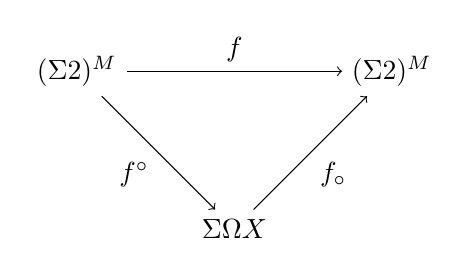
\begin{tikzpicture}[node distance=2cm, auto]
  \node (A) {$(\Sigma 2)^M$};
  
  \node (C) [right of=A, below of=A] {$\Sigma\Omega X$};
  \node (B) [right of=C, above of =C ] {$(\Sigma 2)^M$};
  \draw[->] (A) to node {$f$} (B);
  \draw[->] (A) to node [swap] {$f^\circ$} (C);
  \draw[->] (C) to node [swap] {$f_\circ$} (B);
\end{tikzpicture}
 \end{center}
 of continuous maps. Since $f_\circ: X \to (\Sigma 2)^M$ is an embedding, then the identity map $\text{id}_X: \Sigma\Omega X \to X$ is continuous. Since the retraction $f^\circ: (\Sigma 2)^M \to X$ is a quotient map (as all retractions are), the identity map in the other direction $\text{id}_X: X \to \Sigma\Omega X$ is continuous. This proofs that $\text{id}_X$ is a homeomorphism. Hence $\Sigma\Omega X = X$.
\end{proof}

There is, therefore, a canonical bijection between continuous lattices and injective topological $T_0$-spaces. In fact we have shown that $INJ$, the full subcategory of $TOP$ consisting of injective spaces and all continuous maps, is essentially the same category as $CONT$. This allows not only a purely topological description of continuous lattices (injective spaces under the specialization order), but also a complete answer to the question whcih spaces are of the form $\Sigma L$ with $L$ continuous. We conclude this paper with a resume of the principial results of this subsection:

\begin{theorem}
\begin{enumerate}[(i)]
  \item If $L$ is a continuous lattice, then $\Sigma L = (L, \sigma(L))$ is an injective space and $\Omega\Sigma L = L$.
  \item If $X$ is an injective $T_0$-space, then $\Omega X = (X, \leq)$ is a continuous lattice (with respect to the specialization order) and $\Sigma\Omega X = X$.
\end{enumerate}
\end{theorem}

\newpage

\begin{thebibliography}{99}
\bibitem{1} G. Gierz, K. H. Hofmann, K. Keimel, J. D. Lawson, M. W. Mislove, D. S. Scott, {\em Continuous Lattices and Domains}, Cambridge University Press, Cambridge (2003).
\bibitem{2} E. Colebunders, \emph{Topologie}, Vrije Universiteit Brussel, 2012.
\bibitem{3} K. Martin, \emph{A Foundation for Computation}, July 2000
\bibitem{4} J.Goubault-Larrecq, \emph{Non-Hausdorff Topology and Domain Theory}, Cambridge University Press, 2013.
\bibitem{5} S. Abramsky, Dov M. Gabbay, T. S. E. Maibaum, \emph{Handbook for Logic in
Computer Science}, Clarendon Press Oxford, 1994.
    \end{thebibliography}
\end{document}

